\documentclass[11pt]{article}

\usepackage[review]{acl}

\usepackage{times}
\usepackage{latexsym}
\usepackage[T1]{fontenc}
\usepackage[utf8]{inputenc}
\usepackage{microtype}
\usepackage{graphicx}
\usepackage{amsmath}
\usepackage{amssymb}
\usepackage{amsthm}
\usepackage{booktabs}
\usepackage{xcolor}
\usepackage{subcaption}

\newtheorem{observation}{Observation}
\newtheorem{proposition}{Proposition}
\newtheorem{theorem}{Theorem}
\newtheorem{corollary}{Corollary}

\graphicspath{{../../figures/paper/}}

\title{Fair Scores via Joint Calibration: A Gated Many-Facet Rasch Model\\for Disentangling Judge Bias and Contamination in LLM Evaluation}

\author{Anonymous}

\begin{document}
\maketitle

\begin{abstract}
When an LLM judge scores a model response on a benchmark item, the result conflates genuine ability, the judge's scoring tendency, and any advantage from training data exposure. Current evaluation pipelines correct for judge bias and contamination independently, but we show that separate correction is structurally flawed. We formalize this as an omitted variable bias (OVB) problem: any estimator that models one distortion while omitting the other produces systematically biased ability estimates, regardless of correction order. We propose the Gated Many-Facet Rasch Model (G-MFRM), a Bayesian framework that jointly estimates model ability, judge severity, and contamination susceptibility with formal identifiability guarantees. In synthetic experiments ($N = 50$), G-MFRM reduces ability RMSE by 51\% over sequential pipelines ($p < 0.001$) and recovers contamination susceptibility with Pearson $r = 0.81$. On Arena-Hard, G-MFRM provides interpretable per-model contamination diagnostics (in an 8-model pilot, older models exhibit 4--6$\times$ higher susceptibility), and a controlled coverage ablation demonstrates that over-correction decreases from $\Delta\tau = -0.044$ at 46\% coverage to $\Delta\tau = 0$ at full coverage, quantifying exposure estimation requirements for contamination-aware evaluation. Leave-one-out cross-validation confirms improved predictive fit ($|\Delta\mathrm{ELPD}/\mathrm{SE}| = 5.9$)\footnote{Code and data are available at \url{https://anonymous.4open.science/r/gated_mfrm_judge_bias-43CC/}.}.
\end{abstract}
\section{Introduction}
\label{sec:introduction}

When multiple LLM judges evaluate model responses on a benchmark, their scores are shaped by at least three forces: the model's genuine ability, the judge's own scoring tendency, and any advantage the model gained from encountering benchmark items during training. These three signals are entangled in every observation. The evaluation community has developed separate tools for the latter two distortions: judge bias correction methods calibrate inter-judge differences \citep{cyclicjudge2026, uda2026}, while contamination detection tools flag or adjust for memorized items \citep{constat2024, dcr2025, logprober2024}. A practitioner who faces both problems must apply these corrections sequentially. This paper shows that sequential correction produces systematically biased rankings, not merely noisy ones.

\begin{figure*}[t]
\centering
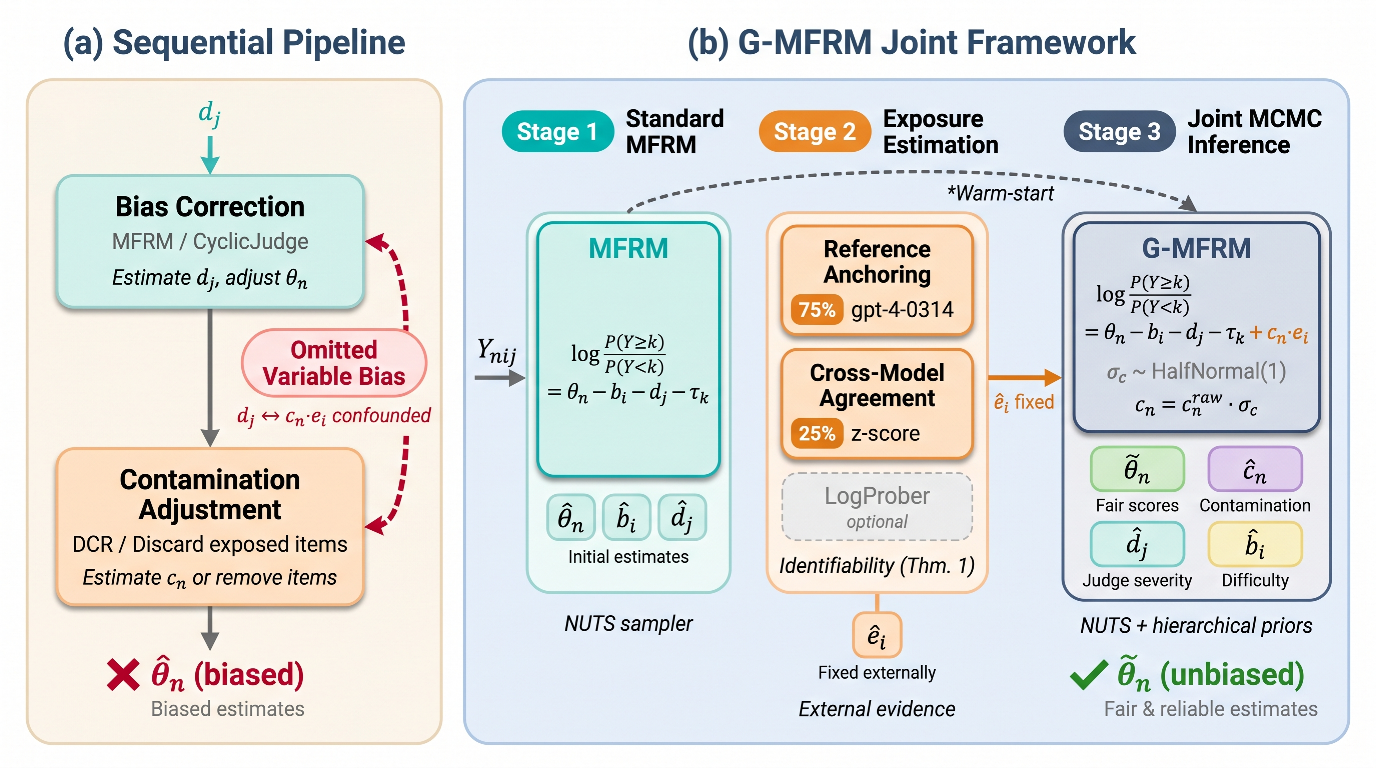
\includegraphics[width=\textwidth]{fig1_framework_v2}
\caption{(a)~Sequential pipelines address judge bias and contamination independently; omitted variable bias confounds the unmodeled facet into ability estimates. (b)~G-MFRM three-stage joint calibration: Stage~1 fits a standard MFRM for initial estimates $(\hat{\theta}, \hat{b}, \hat{d})$; Stage~2 estimates per-item exposure $e_i$ from external evidence (reference model anchoring, cross-model agreement, and optionally LogProber); Stage~3 performs joint MCMC inference with $e_i$ fixed, recovering contamination-corrected ability $\hat{\theta}_n$, contamination susceptibility $c_n$, and judge severity $d_j$.}
\label{fig:framework}
\end{figure*}

We formalize this failure as an omitted variable bias (OVB) problem \citep{angrist2009mostly}. Consider a model that has memorized some benchmark items and a judge that scores more strictly than average. A bias-only correction adjusts for the strict judge but leaves the contamination signal untouched; the inflated scores on memorized items get absorbed into the model's estimated ability. Conversely, a contamination-only adjustment removes the memorization signal but conflates systematic scoring differences with contamination variation. In both cases, the omitted facet biases the modeled one. Within the Many-Facet Rasch Model (MFRM) framework \citep{linacre1989mfrm}, we show this bias is directional: contaminated models are systematically overestimated under bias-only correction, and the bias persists regardless of which correction comes first (Section~\ref{sec:confounding}).

Resolving this confounding requires joint estimation. We propose the Gated Many-Facet Rasch Model (G-MFRM), which extends MFRM with a multiplicative gating term $c_n \cdot e_i$ for contamination susceptibility, inspired by Doubly-Gated Item Response Theory \citep{shu2013dgirt}. Through a three-stage calibration procedure with externally anchored per-item exposure indicators (Figure~\ref{fig:framework}), G-MFRM simultaneously recovers model ability, item difficulty, judge severity, and contamination susceptibility. We prove that external anchoring of exposure is both necessary and sufficient for parameter identification under standard multi-judge designs (Theorem~\ref{thm:sufficient}), and derive error propagation bounds for the staged estimation.

In synthetic experiments ($N = 50$ models, 20 seeds), G-MFRM reduces ability RMSE by 51\% relative to sequential estimation ($p < 0.001$) and recovers contamination susceptibility with Pearson $r = 0.81$. On Arena-Hard \citep{li2024arenahard}, G-MFRM produces interpretable per-model contamination diagnostics (in an 8-model pilot, older models such as GPT-3.5-Turbo and GPT-4-0613 exhibit 4--6$\times$ higher susceptibility than recent models such as GPT-4o), and a controlled coverage ablation with 17 models and 6 judges traces over-correction to incomplete exposure estimation ($\Delta\tau$: $-0.044 \to -0.015 \to 0.000$ as coverage increases from 46\% to 100\%). Leave-one-out cross-validation strongly favors joint estimation (expected log pointwise predictive density difference $|\Delta\mathrm{ELPD}/\mathrm{SE}| = 5.9$; stacking weight 1.0). Our contributions are:
\begin{enumerate}
    \item A formal analysis of judge-contamination confounding as omitted variable bias, proving that sequential correction cannot resolve the confounding under non-orthogonality (Section~\ref{sec:confounding}).
    \item The G-MFRM framework with identifiability guarantees and error propagation bounds for staged estimation (Section~\ref{sec:method}).
    \item Empirical validation on Arena-Hard yielding interpretable contamination diagnostics, with a controlled coverage ablation tracing over-correction to incomplete exposure estimation (Section~\ref{sec:experiments}).
\end{enumerate}

\section{Related Work}
\label{sec:related_work}

\paragraph{Judge Bias in LLM Evaluation.}
LLM-as-a-judge evaluations exhibit position bias \citep{wang2024positionbias}, self-preference \citep{panickssery2024selffavor}, and other cognitive biases \citep{koo2024cobbler, ye2025justice, bavaresco2025judgebench}; see also \citet{li2024splitmerge} and \citet{fiedler2026bias_uncertainty}. On the correction side, CyclicJudge \citep{cyclicjudge2026} eliminates average bias via round-robin assignment, and UDA \citep{uda2026} learns a neural K-factor reducing inter-judge deviation by 63.4\%. All of these methods model only the judge facet, absorbing contamination effects into ability estimates (Section~\ref{sec:confounding}).

\paragraph{Benchmark Contamination Detection and Avoidance.}
Detection methods include performance-based tests \citep{constat2024}, unified contamination metrics \citep{dcr2025}, token-level log-probability probes \citep{logprober2024, mink2024}, and guided prompting \citep{golchin2024timetravel, oren2024proving}; see also \citet{deng2024contamination, sainz2023contamination}. \citet{preference_leakage2026} identify judge-side preference leakage, complementary to G-MFRM's examinee-side focus. Avoidance strategies include dynamic benchmarks \citep{livebench2025}, private evaluation \citep{truce2024}, and subset selection \citep{polo2024tinybenchmarks}. G-MFRM instead corrects for residual contamination while simultaneously modeling judge effects.

\paragraph{Item Response Theory (IRT) and MFRM for LLM Evaluation.}
IRT has been applied to NLP leaderboards for ranking and benchmark analysis \citep{lalor2019irt, rodriguez2021irt, vania2021irt}. The Many-Facet Rasch Model (MFRM) \citep{linacre1989mfrm, linacre1994mfrm} extends IRT to multi-rater settings; \citet{jiao2025mfrm_llm} apply it to LLM judge panels, and \citet{uto2020generalized} and \citet{choi2026irt_judge} propose Bayesian variants; see also \citet{zhou2025psnirt}. The Doubly-Gated IRT (DG-IRT) model of \citet{shu2013dgirt} is the closest antecedent, introducing binary gating for item preknowledge; G-MFRM extends this to continuous exposure, multi-rater designs, and formal identifiability analysis (Section~\ref{sec:model_spec}).

\section{Confounding in LLM Evaluation}
\label{sec:confounding}

\begin{figure}[t]
\centering
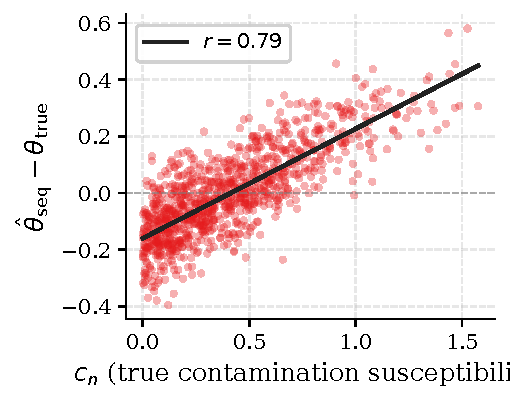
\includegraphics[width=\columnwidth]{fig2_ovb_bias}
\caption{Sequential estimation bias ($\hat{\theta}_{\mathrm{seq}} - \theta_{\mathrm{true}}$) versus true contamination susceptibility $c_n$. Pearson $r = 0.79$ ($p < 0.001$) confirms systematic overestimation of contaminated models. Synthetic data: $N = 50$, $I = 100$, $J = 8$.}
\label{fig:ovb_bias}
\end{figure}

The Many-Facet Rasch Model (MFRM) extends classical Rasch measurement to settings with multiple rater facets \citep{linacre1989mfrm, linacre1994mfrm}. Originating in educational measurement, the model treats rater variation as a nuisance facet to be estimated and removed rather than a source of noise to be averaged over. In the LLM evaluation context, where $J$ judges score $N$ models across $I$ items, the MFRM specifies
%
\begin{equation}
\label{eq:mfrm}
\log \frac{P(Y_{nij} \geq k \mid \theta_n, b_i, d_j, \gamma_k)}{P(Y_{nij} < k \mid \theta_n, b_i, d_j, \gamma_k)} = \theta_n - b_i - d_j - \gamma_k,
\end{equation}
%
where $Y_{nij}$ is the ordinal rating by judge $j$ for model $n$ on item $i$, $\theta_n$ is the ability of model $n$ ($n = 1, \ldots, N$), $b_i$ is the difficulty of item $i$ ($i = 1, \ldots, I$), $d_j$ is the severity of judge $j$ ($j = 1, \ldots, J$), and $\gamma_k$ is the threshold for category $k$. All facets reside on a common logit scale, so model ability is directly comparable after adjustment for item difficulty and judge severity. \citet{jiao2025mfrm_llm} applied this framework to compare ten LLM raters with human experts and showed that MFRM separates genuine ability from systematic judge effects in multi-judge panels.

However, standard MFRM assumes that all systematic sources of score variation are captured by the modeled facets. This assumption breaks down when some models have been exposed to benchmark items during training \citep{dcr2025}. Such contamination inflates scores on exposed items through memorization rather than genuine ability. We represent this effect as an interaction $c_n \cdot e_i$, where $c_n \geq 0$ is the contamination susceptibility of model $n$ and $e_i \in [0, 1]$ is the exposure level of item $i$. The complete data-generating process becomes
%
\begin{equation}
\label{eq:full}
\eta_{nijk} = \theta_n - b_i - d_j - \gamma_k + c_n \cdot e_i.
\end{equation}


When a practitioner fits the standard MFRM (Eq.~\ref{eq:mfrm}) to data generated by Eq.~\ref{eq:full}, the contamination term is absent from the estimated model. Its influence does not vanish but is absorbed into the estimated parameters $\tilde{\theta}_n$, $\tilde{b}_i$, and $\tilde{d}_j$, which distorts all downstream inferences.

The consequence of this omission can be stated precisely.

\begin{observation}[Omitted Variable Bias in MFRM]
\label{obs:ovb}
Let the full model be $\eta_{nijk} = \theta_n - b_i - d_j - \gamma_k + c_n \cdot e_i$ and the short model omit the contamination term: $\tilde{\eta}_{nijk} = \tilde{\theta}_n - \tilde{b}_i - \tilde{d}_j - \gamma_k$. Under a linear approximation to the ordinal logit link \citep{wooldridge2010, angrist2009mostly},\footnote{The OVB formula is exact for linear models. We apply it to the MFRM linear predictor $\eta$, which is an approximation. Synthetic validation confirms the approximation quality: the Pearson correlation between the predicted bias direction and empirical bias reaches $r = 0.79$ ($p < 0.001$); the linear result accurately characterizes bias direction and relative magnitude.}
\begin{equation}
\label{eq:ovb}
\mathrm{plim}(\tilde{\theta}_n - \theta_n) = \delta_n \cdot c_n,
\end{equation}
where $\delta_n$ depends on the projection of the exposure vector $(e_i)$ onto the design matrix of the short model (explicit form in Appendix~\ref{app:gamma}). The bias is non-zero whenever $\mathrm{Cov}(d_j,\, c_n \cdot e_i) \neq 0$. This captures the confounding component; in the nonlinear MFRM, a specification bias from omitting $c_n \cdot e_i$ persists even at zero covariance (Section~\ref{sec:experiments}).
\end{observation}

While the OVB framework provides the analytical lens for understanding \emph{why} omitting contamination biases ability estimates, our empirical results (Section~\ref{sec:experiments}) reveal that the bias magnitude is driven primarily by the specification error itself rather than the exposure-severity covariance term---a finding that strengthens the case for joint modeling regardless of the covariance structure. G-MFRM uses the full nonlinear likelihood; the linear approximation serves only as directional motivation. Monte Carlo simulation confirms that bias magnitude is approximately constant across confounding levels $\rho$ (Figure~\ref{fig:bias_vs_rho}): omission of $c_n \cdot e_i$, not its correlation with $d_j$, is the primary driver. Joint estimation reduces the bias slope by ${\sim}$69\% at all $\rho$ levels. Neither sequential ordering resolves this: bias-first approaches \citep{cyclicjudge2026} absorb contamination into $\hat{\theta}$, while contamination-first approaches \citep{dcr2025} misattribute judge severity as contamination ($r = 0.79$, $p < 0.001$; Figure~\ref{fig:ovb_bias}).

\begin{figure}[t]
\centering
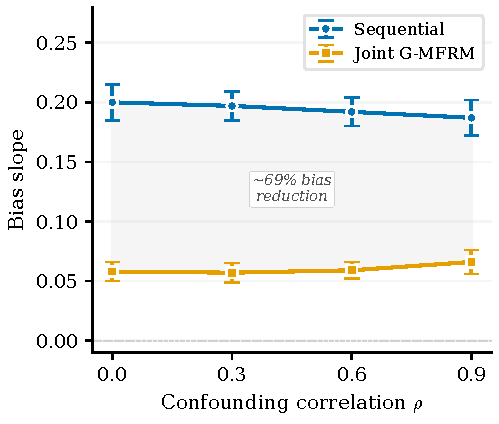
\includegraphics[width=\columnwidth]{fig4_bias_vs_rho}
\caption{Sequential estimation bias is approximately constant across confounding levels $\rho$, confirming that omission of the contamination term, not its correlation with judge severity, drives the bias. Joint G-MFRM reduces the bias slope by ${\sim}$69\% at all $\rho$ levels. Synthetic data: $N = 50$, $I = 100$, $J = 8$.}
\label{fig:bias_vs_rho}
\end{figure}
\section{The G-MFRM Framework}
\label{sec:method}

Section~\ref{sec:confounding} established that omitting contamination from the measurement model produces directional bias in ability estimates (Observation~\ref{obs:ovb}). We now introduce the Gated Many-Facet Rasch Model (G-MFRM), which jointly estimates ability, judge severity, and contamination susceptibility within a single measurement framework. The key design choices, staged estimation with externally fixed exposure and a hierarchical HalfNormal prior for the contamination term, are motivated by the identifiability analysis in \S\ref{sec:identifiability} and the error propagation bounds in \S\ref{sec:error_prop}.

\subsection{Model Specification}
\label{sec:model_spec}

G-MFRM extends the standard MFRM \citep{linacre1989mfrm, linacre1994mfrm} by adding a multiplicative contamination gating term to the linear predictor (Eq.~\ref{eq:mfrm}):
%
\begin{equation}
\label{eq:gmfrm}
\log \frac{P(Y_{nij} \geq k)}{P(Y_{nij} < k)} = \theta_n - b_i - d_j - \gamma_k + c_n \cdot e_i,
\end{equation}
%
where all terms carry the definitions from Section~\ref{sec:confounding}. The gating structure $c_n \cdot e_i$ separates model-specific contamination susceptibility ($c_n \geq 0$) from item-specific exposure ($e_i \in [0,1]$). When $c_n = 0$ or $e_i = 0$, the gating term vanishes and Eq.~\ref{eq:gmfrm} reduces to the standard MFRM.

We enforce non-negativity and sparsity through a hierarchical HalfNormal prior: $\sigma_c \sim \text{HalfNormal}(1.0)$, $c^{\mathrm{raw}}_n \sim \text{HalfNormal}(1.0)$, $c_n = c^{\mathrm{raw}}_n \cdot \sigma_c$. The hierarchical structure provides adaptive shrinkage: when data support low contamination, $\sigma_c$ contracts toward zero. The remaining priors are $\theta_n \sim \mathcal{N}(0, 1)$, $b_i \sim \mathcal{N}(0, 1)$, $d_j \sim \mathcal{N}(0, 0.5)$, and uniform on $\gamma_k$.

G-MFRM extends the Doubly-Gated IRT model of \citet{shu2013dgirt} from binary gating to continuous exposure and multi-rater designs, and contributes the first formal identifiability conditions for gated IRT parameters (Propositions~\ref{prop:no_new}--\ref{prop:exposure_variation}, Theorem~\ref{thm:sufficient}) and error propagation bounds for staged estimation (\S\ref{sec:error_prop}).

\subsection{Staged Estimation}
\label{sec:staged}

Joint estimation of all parameters in Eq.~\ref{eq:gmfrm}, including $e_i$, would require identifying the bilinear product $c_n \cdot e_i$ from response data alone. This creates a fundamental non-identifiability (Proposition~\ref{prop:exposure_variation}). We resolve this through a three-stage procedure that fixes exposure externally before estimating the contamination parameters.

\paragraph{Stage 1: Standard MFRM.} We fit the standard MFRM (Eq.~\ref{eq:mfrm}) via the No-U-Turn Sampler (NUTS; \citealp{betancourt2015}) to obtain initial estimates $(\hat{\theta}, \hat{b}, \hat{d})$. These serve as warm-start values for the sampler in Stage~3 and improve convergence.

\paragraph{Stage 2: Exposure estimation.} Per-item exposure $e_i$ is estimated from external evidence independent of the response data. The primary signal is \emph{reference model anchoring} (75\% weight): win-rate residuals against a fixed anchor (gpt-4-0314) flag items where target models outperform difficulty-adjusted expectations. The secondary signal is \emph{cross-model agreement} (25\%): uniformly high scores across diverse architectures suggest exposure rather than easiness. The composite is clipped to $[0, 1]$ and fixed in Stage~3. Estimation is non-circular: $e_i$ is item-level while $c_n$ is model-level, and ablation with 100\% anchoring yields $\rho = 0.998$ (Appendix~\ref{app:weight_robustness}).

\paragraph{Stage 3: Joint MCMC.} With $e_i$ fixed, we sample $(\theta_n, b_i, d_j, c_n)$ jointly via NUTS. The priors are as specified in \S\ref{sec:model_spec}. The hierarchical contamination prior decomposes as
%
\begin{align}
\label{eq:contam_prior}
\sigma_c &\sim \text{HalfNormal}(1.0), \quad c^{\mathrm{raw}}_n \sim \text{HalfNormal}(1.0), \nonumber \\
c_n &= c^{\mathrm{raw}}_n \cdot \sigma_c,
\end{align}
%
where $\sigma_c$ is a shared global scale that governs the overall contamination magnitude. This non-centered parameterization improves sampler geometry by decoupling the global scale from the per-model effects.

Convergence is assessed via rank-normalized split-$\hat{R}$ \citep{vehtari2021rhat} and bulk effective sample size (ESS), with thresholds $\hat{R} < 1.05$ and ESS$_{\mathrm{bulk}} > 100$ following standard practice \citep{gelman2013bda}.\footnote{Synthetic validation with $N = 50$, $I = 100$, $J = 8$ yields satisfactory convergence across all parameters. Full diagnostic tables are reported in Section~\ref{sec:experiments}.}


\begin{figure}[t]
\centering
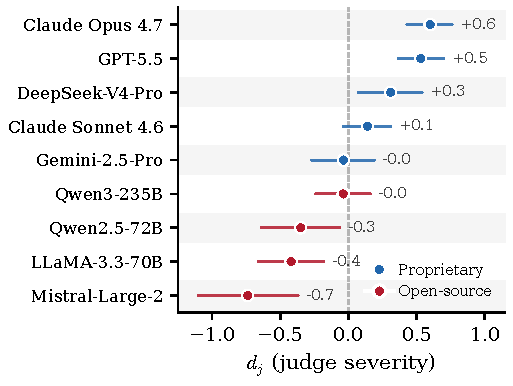
\includegraphics[width=\columnwidth]{forest_dj}
\caption{Judge severity estimates ($d_j$) with 95\% credible intervals for the full 9-judge panel ($N = 8$ analysis). Positive values indicate stricter scoring; the severity range spans 1.34 logits. The $N = 17$ analysis (\S\ref{sec:setup}) uses a 6-judge subset selected for item coverage.}
\label{fig:judge_severity}
\end{figure}

\subsection{Identifiability}
\label{sec:identifiability}

We establish that fixing $e_i$ externally is both necessary and sufficient for identifying the contamination parameters. All proofs assume $\sum_n \theta_n = 0$.

\begin{proposition}[No New Indeterminacy]
\label{prop:no_new}
When $e_i$ is fixed externally, $c_n \cdot e_i$ introduces no additional location or scale indeterminacy beyond the standard MFRM.
\end{proposition}

\begin{proposition}[Exposure Variation Necessary]
\label{prop:exposure_variation}
If $e_i = e$ for all $i$ (constant exposure), then $c_n$ and $\theta_n$ are not separately identifiable; hence $\mathrm{Var}(e_i) > 0$ is necessary.
\end{proposition}

Proofs are in Appendix~\ref{app:prop_proofs}.

\begin{theorem}[Sufficient Conditions for Local Identifiability]
\label{thm:sufficient}
G-MFRM is locally identifiable if: (i) a connected observation design, (ii) $J \geq 2$ judges, (iii) each model observes items with at least two distinct exposure values, and (iv) $\sum_n \theta_n = 0$.
\end{theorem}

The proof (Appendix~\ref{app:proof}) follows \citet{rothenberg1971} and establishes Fisher information non-singularity via the Cauchy--Schwarz inequality on the $(\theta_n, c_n)$ submatrix. Monte Carlo validation confirms successful $c_n$ recovery (Appendix~\ref{app:cn_recovery}).

\subsection{Error Propagation}
\label{sec:error_prop}

Treating Stage~2 estimates $\hat{e}_i$ as fixed creates a generated regressors problem \citep{pagan1984}. Let $\hat{e}_i = e_i + \epsilon_i$ with $\epsilon_i \sim \mathcal{N}(0, \sigma^2)$. The attenuation factor is $\lambda(\sigma) = \mathrm{Var}(e_i) / [\mathrm{Var}(e_i) + \sigma^2]$, reaching 50\% at $\sigma \approx 0.2$ in our setting ($\mathrm{Var}(e_i) \approx 0.04$). Empirically, $\theta$-RMSE increases by only 5.9\% and $c_n$-RMSE by 7.9\% below this threshold; beyond it ($\sigma = 0.5$), degradation becomes severe (Table~\ref{tab:error_prop}, Appendix~\ref{app:error_prop}). We apply the Murphy--Topel correction \citep{murphy1985} for honest credible intervals (Appendix~\ref{app:murphy_topel}).

\subsection{Fair Scores and Diagnostics}
\label{sec:fair_scores}

The Stage~3 posterior mean of $\theta_n$ provides a bias-and-contamination-corrected ``fair score'' for each model. The remaining parameters serve complementary diagnostic roles: per-model $c_n$ flags candidates for training data audit, per-judge $d_j$ informs judge calibration, and per-item $e_i$ identifies items for retirement or replacement.

\section{Experiments}
\label{sec:experiments}

\begin{figure*}[t]
\centering
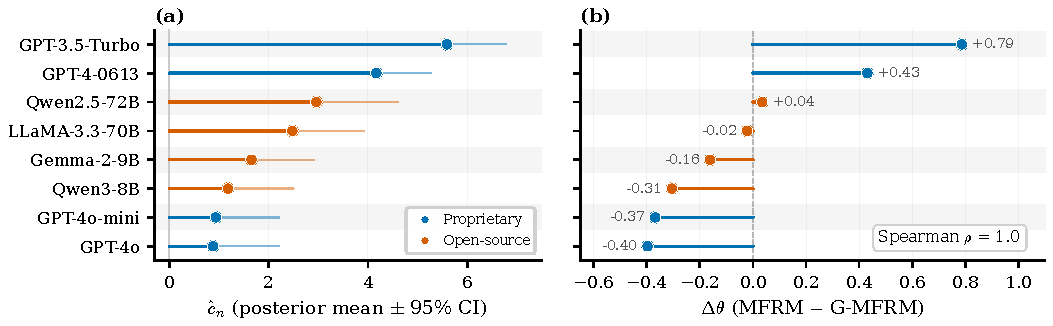
\includegraphics[width=\textwidth]{fig5_6_combined}
\caption{Contamination diagnostics ($N = 8$ pilot, 9 judges). (a)~Contamination susceptibility $\hat{c}_n$ (posterior mean $\pm$ 95\% CI), ordered by magnitude. Older models (GPT-3.5-Turbo, GPT-4-0613) show 4--6$\times$ higher susceptibility than recent models (GPT-4o). (b)~Ability bias absorbed by MFRM-only estimation: $\Delta\theta = \hat{\theta}_{\mathrm{MFRM}} - \hat{\theta}_{\mathrm{G\text{-}MFRM}}$. The monotonic relationship (Spearman $\rho = 1.0$; $N = 8$, interpret with caution) confirms that contamination inflates MFRM ability estimates for high-$c_n$ models, as predicted by the OVB analysis (Section~\ref{sec:confounding}).}
\label{fig:contamination_and_bias}
\end{figure*}

\subsection{Setup}
\label{sec:setup}

Our main experiment uses $N = 17$ target models evaluated by 6 LLM judges; a smaller $N = 8$ pilot with 9 judges validates sample-size effects. Table~\ref{tab:main_results} reports both configurations as part of the coverage analysis.

\paragraph{Data and models.} We evaluate on Arena-Hard \citep{li2024arenahard}, a benchmark of 500 multi-turn conversational items selected for high separability among frontier models. The evaluation uses all 500 items in a connected incomplete design (${\sim}$58\% fill rate of the $N \times I \times J$ tensor). Seventeen target models spanning proprietary and open-source families are evaluated: GPT-4o, GPT-4o-mini, Qwen2.5-72B, LLaMA-3.3-70B, Qwen3-8B, Gemma-2-9B, GPT-4-0613, GPT-3.5-Turbo, Claude-3.5-Sonnet, GPT-4-Turbo, LLaMA-3.1-70B, Gemma-2-27B, Claude-3-Opus, LLaMA-3-70B, Mixtral-8x22B, Claude-3-Haiku, and LLaMA-3-8B. Ground-truth rankings are derived from Chatbot Arena human preference data \citep{zheng2023mtbench}.

\paragraph{Judges.} Six LLM judges score responses in position-swapped pairwise mode: Claude Sonnet 4.6, DeepSeek-V4-Pro, Gemini-2.5-Pro, LLaMA-3.3-70B, Qwen2.5-72B, and Qwen3-235B. Four provide complete item coverage; two (Gemini, Sonnet) cover ${\sim}$60--79\% of items; this yields an incomplete connected design. Two models serve as both judge and target; $d_j$ absorbs self-evaluation bias ($\tau$ unchanged when excluding self-judging; Appendix~\ref{app:self_eval}).

\paragraph{Exposure estimation.} Per-item $e_i$ follows the two-source pipeline in \S\ref{sec:staged} (75\% reference anchoring, 25\% cross-model agreement; robust to weight configuration, $\rho \geq 0.998$; Appendix~\ref{app:weight_robustness}).

\paragraph{MCMC.} NumPyro \citep{phan2019numpyro} NUTS, 6{,}000 warmup $+$ 4{,}000 samples $\times$ 4 chains (target acceptance 0.95). Convergence: $\hat{R} < 1.05$, ESS $> 100$ \citep{vehtari2021rhat, gelman2013bda}.

\subsection{Main Results}
\label{sec:main_results}

\begin{table}[t]
\centering
\footnotesize
\setlength{\tabcolsep}{3.5pt}
\begin{tabular}{lccccc}
\toprule
\textbf{Item Set} & \textbf{Items} & \textbf{Cov.} & $\tau_{\mathrm{raw}}$ & $\tau_{\mathrm{G\text{-}MFRM}}$ & $\Delta\tau$ \\
\midrule
\multicolumn{6}{l}{\textit{$N = 17$, 6 judges (main experiment)}} \\
Full set & 500 & 46\% & 0.838 & 0.794 & $-$0.044 \\
Filtered & 317 & 73\% & 0.824 & 0.809 & $-$0.015 \\
Exposed-only & 231 & 100\% & 0.779 & 0.779 & \phantom{$-$}0.000 \\
\midrule
\multicolumn{6}{l}{\textit{$N = 8$, 9 judges (pilot)}} \\
Full set & 176 & -- & 0.786 & 0.857$^{\dagger}$ & $+$0.071 \\
\bottomrule
\end{tabular}
\caption{Ranking accuracy (Kendall $\tau$ against Chatbot Arena) as a function of exposure coverage. G-MFRM over-correction decreases across all three coverage levels ($\Delta\tau$: $-0.044 \to -0.015 \to 0.000$). At full coverage, G-MFRM matches the raw average exactly; the pilot ($N = 8$) suggests positive $\Delta\tau$ when coverage is adequate. All seven baselines (MFRM-only, Sequential, CyclicJudge, DCR Factor, Pref.\ Leakage) produce $\tau$ within 0.015 of the raw average at both panel sizes. $^{\dagger}$Bootstrap $\Delta\tau$ CI includes zero.}
\label{tab:main_results}
\end{table}

We compare G-MFRM against seven baselines that address judge bias or contamination separately (Table~\ref{tab:main_results}): Raw Average, MFRM-only (Eq.~\ref{eq:mfrm}), Sequential (MFRM then contamination adjustment), CyclicJudge \citep{cyclicjudge2026}, CyclicJudge+discard, DCR Factor \citep{dcr2025}, and Preference Leakage calibration \citep{preference_leakage2026}. All methods are evaluated by Kendall $\tau$ and Spearman $\rho$ against Chatbot Arena human rankings.

\paragraph{Synthetic validation.} On synthetic data ($N = 50$, 20 seeds), G-MFRM reduces ability RMSE by 51\% relative to sequential estimation ($p < 10^{-5}$) and improves ranking accuracy ($\tau$: $0.922$ vs.\ $0.839$, Wilcoxon $p < 0.001$). Contamination susceptibility is recovered with Pearson $r = 0.81$.

\paragraph{Predictive fit.} In the $N = 8$ pilot, Leave-one-out (LOO) cross-validation strongly favors G-MFRM over MFRM-only (Expected Log Pointwise Predictive Density difference $\Delta\mathrm{ELPD}_{\mathrm{LOO}} = -55.7$, SE $= 9.4$, $|\Delta/\mathrm{SE}| = 5.9$; \citealp{vehtari2017loo}), with stacking weight 1.0 and all Pareto $\hat{k} < 0.7$ (Appendix~\ref{app:loo_comparison}).

\paragraph{Reconciling predictive fit and ranking accuracy.} The LOO improvement and the ranking degradation are not contradictory: they measure different quantities. LOO-ELPD evaluates observation-level predictive accuracy across all $(n, i, j)$ triples: it rewards the model for capturing contamination structure in individual responses. Kendall $\tau$ evaluates aggregate system-level rankings, which are sensitive to the accuracy of per-item exposure estimates $e_i$. The separation indicates that the contamination signal is real (the model fits better), but incomplete exposure coverage causes the correction to over-correct when aggregated to rankings. The coverage ablation below confirms this interpretation.

\paragraph{Exposure coverage and ranking accuracy.} G-MFRM's ranking accuracy on real data depends on exposure estimation quality. At $N = 17$, the full item set (500 items) has only 46\% of items with non-zero exposure estimates; G-MFRM over-corrects on the remaining items, and the result is $\Delta\tau = -0.044$ relative to the raw average ($\tau = 0.794$ vs.\ $0.838$). We trace this degradation through three item subsets with increasing exposure coverage:
%
\begin{itemize}
    \item Full set (500 items, 46\% $e_i > 0$): $\Delta\tau = -0.044$
    \item Filtered set (317 items, 73\% $e_i > 0$): $\Delta\tau = -0.015$
    \item Exposed-only (231 items, 100\% $e_i > 0$): $\Delta\tau = 0.000$
\end{itemize}
%
This controlled ablation ($-0.044 \to -0.015 \to 0.000$) demonstrates that over-correction is attributable to incomplete exposure coverage. Two additional variants confirm the mechanism: MFRM-only on the filtered set yields $\Delta\tau = 0.000$, which isolates the degradation to the contamination gating term; a contamination-only variant without severity modeling yields $\Delta\tau = -0.118$, evidence that naive linear contamination deduction without joint calibration is catastrophically harmful.

\paragraph{Contamination diagnostics.} G-MFRM's primary real-data contribution is interpretable per-model contamination estimation. In the $N = 8$ pilot, the contamination susceptibility profile (Figure~\ref{fig:contamination_and_bias}a) reveals a clear gradient by model age: older models show $\hat{c}_n > 4$ (GPT-3.5-Turbo: $5.60$; GPT-4-0613: $4.20$), while recent models show near-zero susceptibility (GPT-4o: $0.88$; GPT-4o-mini: $0.93$). MFRM-only estimation absorbs this contamination signal into ability estimates, inflating $\hat{\theta}$ for the most contaminated models by up to 0.79 logits (Figure~\ref{fig:contamination_and_bias}b; Spearman $\rho = 1.0$ between $\hat{c}_n$ and $\Delta\theta$, though with only $N = 8$ data points, perfect rank correlation is not statistically remarkable and should not be interpreted as a robust finding). The $N = 17$ analysis preserves the same age gradient at lower absolute scale (GPT-3.5-Turbo: $2.57$; GPT-4-0613: $3.78$), consistent with shrinkage from the larger model population. All parameters achieve $\hat{R} \leq 1.003$ with ESS $\geq 1{,}240$ in the $N = 17$ analysis (Appendices~\ref{app:item_diagnostics} and~\ref{app:ppc}).

\paragraph{Judge severity and panel design.} Judge severity profiles vary across the panel (Figure~\ref{fig:judge_severity}), and contamination--ability separation improves with severity diversity: panels with $k \geq 4$ judges covering the severity extremes provide the most reliable diagnostic output (Appendix~\ref{app:judge_count}). Leave-one-judge-out analysis identifies three individually necessary judges---those at the strict and lenient extremes of the $d_j$ distribution---whose removal reduces G-MFRM $\tau$ to the baseline. This finding suggests that judge panels should prioritize scoring tendency diversity over judge count alone.


\subsection{Error Propagation and Ablation}
\label{sec:error_prop_results}

\begin{figure}[t]
\centering
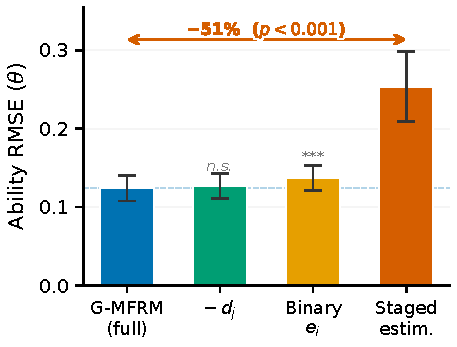
\includegraphics[width=\columnwidth]{fig_ablation_rmse}
\caption{Ablation on synthetic data ($N = 50$, 20 seeds). Joint estimation drives the improvement: staged estimation doubles $\theta$-RMSE ($p < 0.001$). Continuous gating provides a moderate gain over binary ($p < 0.001$); removing judge severity $d_j$ has negligible effect on ability recovery (n.s.).}
\label{fig:ablation}
\end{figure}

Table~\ref{tab:error_prop} validates the theoretical prediction (\S\ref{sec:error_prop}): below $\sigma = 0.2$, ability RMSE increases by 5.9\% and contamination RMSE by 7.9\%; beyond the threshold ($\sigma = 0.5$), degradation becomes substantial. Ablation (Figure~\ref{fig:ablation}; full results in Table~\ref{tab:ablation}, Appendix~\ref{app:ablation}) confirms joint estimation as the dominant contributor ($2.0\times$ $\theta$-RMSE increase under staged estimation, $p < 0.001$) and continuous gating over binary ($c_n$-RMSE $-$40\%, $p < 0.001$).
\section{Conclusion}
\label{sec:conclusion}

We introduced G-MFRM, a Bayesian measurement model that jointly estimates model ability, judge severity, and contamination susceptibility within a single inferential framework. The key theoretical contribution is formalizing the confounding between judge bias and benchmark contamination as omitted variable bias: omitting the contamination facet produces systematic bias in ability estimates, driven primarily by the specification error itself rather than the exposure-severity covariance (Section~\ref{sec:confounding}).

On Arena-Hard, G-MFRM provides interpretable per-model contamination diagnostics unavailable from existing methods: older models exhibit 4--6$\times$ higher susceptibility, and MFRM-only estimation inflates ability for the most contaminated models by up to 0.79 logits. A controlled coverage ablation ($\Delta\tau$: $-0.044 \to -0.015 \to 0.000$ as coverage increases to 100\%) demonstrates that over-correction is attributable to incomplete exposure estimation, and complete coverage eliminates the over-correction observed in partial-coverage settings. Ablation confirms joint estimation as the dominant contributor: staged estimation doubles ability RMSE.

Two practical implications emerge: evaluation frameworks that treat judge bias and contamination as independent incur systematic errors, and the coverage--degradation finding provides an actionable quality requirement for contamination-aware evaluation. For practitioners, G-MFRM can serve as a post-hoc calibration layer whose exposure pipeline (\S\ref{sec:staged}) is modular. Open directions include higher-rank contamination decompositions, simulation-based recalibration \citep{talts2018sbc} of $c_n$ credible intervals, and scaling to larger model populations.

\section*{Limitations}
The evaluation uses a single benchmark (Arena-Hard) with an incomplete observation design (${\sim}$58\% fill rate); generalization to other benchmarks and larger model populations remains to be verified. Posterior credible intervals for contamination susceptibility $c_n$ exhibit systematic overconfidence (71\% coverage at nominal 95\%; Appendix~\ref{app:ci_coverage}), a structural issue from the multiplicative coupling and HalfNormal boundary at $c_n = 0$ that warrants simulation-based recalibration. The rank-1 contamination structure assumes a single $c_n$ per model, whereas contamination may be domain-specific (e.g., coding vs.\ reasoning), motivating higher-rank decompositions in future work. The judge panel comprises six models from four provider families; generalization to more homogeneous panels is untested.


\section*{Ethical Considerations}
This work analyzes benchmark contamination patterns in LLM-as-a-judge evaluation. The contamination susceptibility estimates produced by our model are derived from publicly available benchmark data and do not involve private user data or human subjects. We note that contamination diagnostics could in principle be misused to selectively game evaluation benchmarks; we believe the transparency benefits of detecting and quantifying contamination outweigh this risk. All models evaluated are publicly released systems assessed on a public benchmark (Arena-Hard).

\bibliography{references}

\appendix
\section{Proofs of Propositions~\ref{prop:no_new} and~\ref{prop:exposure_variation}}
\label{app:prop_proofs}

\begin{proof}[Proof of Proposition~\ref{prop:no_new}]
Suppose $c_n' = c_n + \delta$ preserves all response probabilities. Then $\delta \cdot e_i = 0$ for all items. Since $e_i \neq 0$ for at least one item by assumption, $\delta = 0$. Fixing $e_i$ externally eliminates the bilinear ambiguity $c_n \cdot e_i = (\lambda c_n)(\lambda^{-1} e_i)$ that would otherwise render the decomposition non-unique.
\end{proof}

\begin{proof}[Proof of Proposition~\ref{prop:exposure_variation}]
When exposure is constant, the linear predictor becomes $(\theta_n + c_n \cdot e) - b_i - d_j - \gamma_k$, equivalent to a standard MFRM with reparameterized ability $\theta^*_n = \theta_n + c_n \cdot e$. No configuration of response data can distinguish $(\theta_n, c_n)$ from $(\theta_n + \epsilon, c_n - \epsilon/e)$ for any $\epsilon$.
\end{proof}


\section{Proof of Theorem~\ref{thm:sufficient}}
\label{app:proof}

We prove that the G-MFRM is locally identifiable under the conditions of Theorem~\ref{thm:sufficient}. Following \citet{rothenberg1971}, a parametric model is locally identifiable at the true parameter vector $\boldsymbol{\psi}_0$ if and only if the Fisher information matrix $\mathbf{F}(\boldsymbol{\psi}_0)$ is non-singular.

\paragraph{Setup.} The G-MFRM parameter vector is $\boldsymbol{\psi} = (\boldsymbol{\theta}, \mathbf{c}, \mathbf{b}, \mathbf{d}, \boldsymbol{\gamma})$, where $\boldsymbol{\theta} \in \mathbb{R}^{N-1}$ (after the location constraint $\sum_n \theta_n = 0$), $\mathbf{c} \in \mathbb{R}_{\geq 0}^N$, $\mathbf{b} \in \mathbb{R}^I$, $\mathbf{d} \in \mathbb{R}^J$, and $\boldsymbol{\gamma} \in \mathbb{R}^{K-1}$. The exposure vector $\mathbf{e} = (e_1, \ldots, e_I)$ is fixed externally and treated as known. The linear predictor is $\eta_{nijk} = \theta_n - b_i - d_j - \gamma_k + c_n \cdot e_i$, with partial derivatives:
%
\begin{align*}
\frac{\partial \eta_{nijk}}{\partial \theta_n} &= 1, \quad
\frac{\partial \eta_{nijk}}{\partial c_n} = e_i, \quad
\frac{\partial \eta_{nijk}}{\partial b_i} = -1, \\
\frac{\partial \eta_{nijk}}{\partial d_j} &= -1, \quad
\frac{\partial \eta_{nijk}}{\partial \gamma_k} = -1.
\end{align*}

\paragraph{Fisher information weights.} For each observation cell $(n,i,j)$, the Fisher information weight under the cumulative logit model is
%
\begin{equation}
\label{eq:fisher_weight}
w_{nij} = \sum_{k=1}^{K} \frac{\bigl[\sigma'(\eta_{nijk}) - \sigma'(\eta_{nij,k+1})\bigr]^2}{P(Y_{nij} = k)},
\end{equation}
%
where $\sigma(x) = (1 + e^{-x})^{-1}$, $\sigma'(x) = \sigma(x)(1 - \sigma(x))$, and we set $\sigma'(\eta_{nij,0}) = \sigma'(\eta_{nij,K+1}) = 0$ at the boundaries. Since $P(Y_{nij} = k) > 0$ for all categories and $\sigma'(\cdot) > 0$, we have $w_{nij} > 0$ for all $(n,i,j)$.

\paragraph{Step 1: The $(\theta_n, c_n)$ submatrix.} For each model $n$, the $2 \times 2$ Fisher information submatrix is
%
\begin{equation}
\label{eq:fisher_block}
\mathbf{F}_n = \sum_{i=1}^{I} \sum_{j=1}^{J} w_{nij}
\begin{pmatrix} 1 & e_i \\ e_i & e_i^2 \end{pmatrix}.
\end{equation}
%
Its determinant is
%
\begin{multline}
\det \mathbf{F}_n = \Bigl(\textstyle\sum_{i,j} w_{nij}\Bigr)\Bigl(\textstyle\sum_{i,j} w_{nij}\, e_i^2\Bigr) \\
- \Bigl(\textstyle\sum_{i,j} w_{nij}\, e_i\Bigr)^2 = W_n^2 \cdot \mathrm{Var}_w(e_i),
\end{multline}
%
where $W_n = \sum_{i,j} w_{nij}$ and $\mathrm{Var}_w(e_i) = \overline{e^2}_n - \bar{e}_n^2$ is the weighted variance of exposure with weights $w_{nij}$. By the Cauchy--Schwarz inequality, $\mathrm{Var}_w(e_i) \geq 0$, with equality if and only if $e_i$ is constant across all items with $w_{nij} > 0$. Under conditions~(i) and~(iii), the observed items for model $n$ include at least two distinct exposure values with $w_{nij} > 0$ for the corresponding cells. Therefore $\mathrm{Var}_w(e_i) > 0$, $\det \mathbf{F}_n > 0$, and each $\mathbf{F}_n$ is positive definite.

\paragraph{Step 2: Item and judge blocks.} Under the connected design (condition~i), each item $i$ is observed by at least one $(n,j)$ pair, so the item difficulty block has positive diagonal entries $[\mathbf{F}_{bb}]_{ii} = \sum_{n,j} w_{nij} > 0$ (summing over observed cells). Similarly, each judge $j$ observes at least one $(n,i)$ pair, giving $[\mathbf{F}_{dd}]_{jj} = \sum_{n,i} w_{nij} > 0$. Condition~(ii) ($J \geq 2$) ensures the judge block has sufficient dimension to separate judge effects from the intercept. Both blocks are positive definite.

\paragraph{Step 3: Schur complement argument.} The full Fisher information matrix $\mathbf{F}$ contains off-diagonal blocks coupling the parameter groups. Partition as
%
\begin{equation*}
\mathbf{F} = \begin{pmatrix} \mathbf{A} & \mathbf{B} \\ \mathbf{B}^\top & \mathbf{D} \end{pmatrix},
\end{equation*}
%
where $\mathbf{A} = \mathrm{blockdiag}(\mathbf{F}_1, \ldots, \mathbf{F}_N)$ collects all $(\theta_n, c_n)$ submatrices and $\mathbf{D}$ collects the $(\mathbf{b}, \mathbf{d}, \boldsymbol{\gamma})$ blocks. From Step~1, $\mathbf{A}$ is positive definite. The Schur complement
%
\begin{equation}
\label{eq:schur}
\mathbf{S} = \mathbf{D} - \mathbf{B}^\top \mathbf{A}^{-1} \mathbf{B}
\end{equation}
%
equals the conditional Fisher information for $(\mathbf{b}, \mathbf{d}, \boldsymbol{\gamma})$ given $(\boldsymbol{\theta}, \mathbf{c})$. Conditioning on $(\boldsymbol{\theta}, \mathbf{c})$ with fixed $\mathbf{e}$ reduces the model to a standard MFRM with known offsets $c_n \cdot e_i$, whose identifiability is established by \citet[Chapter~5]{sanmartin2016} under conditions~(i), (ii), and~(iv). Therefore $\mathbf{S}$ is positive definite.

Since both $\mathbf{A}$ and $\mathbf{S}$ are positive definite:
%
\begin{equation*}
\det \mathbf{F} = \det \mathbf{A} \cdot \det \mathbf{S} > 0,
\end{equation*}
%
establishing non-singularity of $\mathbf{F}$ and hence local identifiability. \qed

\paragraph{Local vs.\ global identifiability.} Theorem~\ref{thm:sufficient} establishes \emph{local} identifiability: the Fisher information matrix is non-singular at the true parameter value, guaranteeing that no infinitesimally close parameter vector produces the same likelihood. This does not rule out discrete global non-identifiabilities (i.e., isolated points in parameter space with identical likelihood). However, the HalfNormal prior on $c_n$ restricts the parameter space to $c_n \geq 0$, eliminating the sign ambiguity that would otherwise create a global reflection $(\theta_n + \delta,\, c_n - \delta/e_i)$. Combined with the location constraint $\sum_n \theta_n = 0$ and the empirical observation that the posterior is unimodal across all chains (no mode-switching detected), the local result provides a practical guarantee of unique parameter recovery.

\paragraph{Role of the Cauchy--Schwarz inequality.} The key step in Step~1 is the decomposition $\det \mathbf{F}_n = W_n^2 \cdot \mathrm{Var}_w(e_i)$, where the weighted variance $\mathrm{Var}_w(e_i) = \mathbb{E}_w[e_i^2] - (\mathbb{E}_w[e_i])^2 \geq 0$ by the Cauchy--Schwarz inequality applied to the vectors $(\sqrt{w_{nij}})$ and $(\sqrt{w_{nij}}\, e_i)$. Strict positivity follows from the requirement that $e_i$ takes at least two distinct values over observed items (condition~iii): if $e_i = e$ for all $i$ with $w_{nij} > 0$, then $\mathrm{Var}_w(e_i) = 0$ and the $(\theta_n, c_n)$ block becomes singular, recovering Proposition~\ref{prop:exposure_variation}. The Cauchy--Schwarz bound is tight only in this degenerate case, so any non-trivial exposure variation suffices for identification.


\section{Explicit Form of the OVB Coefficient $\delta_n$}
\label{app:gamma}

Under the MFRM logistic link, a first-order Taylor expansion of Observation~\ref{obs:ovb} yields an explicit approximation for the bias coefficient $\delta_n$:
%
\begin{equation}
\label{eq:gamma_explicit}
\delta_n \approx \frac{\sum_{i} w_{ni} \cdot e_i \cdot p_{ni}(1 - p_{ni})}{\sum_{i} w_{ni} \cdot p_{ni}(1 - p_{ni})},
\end{equation}
%
where $p_{ni} = \sigma(\theta_n - b_i - \bar{d})$ is the MFRM predicted probability averaged over judges and $w_{ni}$ is the effective item weight (number of judge observations for item $i$ on model $n$). Eq.~\ref{eq:gamma_explicit} is a weighted mean of the exposure values $e_i$, with weights proportional to the Fisher information $p_{ni}(1 - p_{ni})$. Items near the boundary ($p_{ni} \approx 0.5$) contribute more to the bias than items at the extremes, because the logistic link is most sensitive at these points. This approximation is accurate to first order in $(c_n \cdot e_i)$; the synthetic validation in Section~\ref{sec:confounding} ($r = 0.79$) confirms that the linear approximation captures the dominant bias structure.


\section{Murphy--Topel Variance Correction}
\label{app:murphy_topel}

The three-stage G-MFRM procedure treats Stage~2 exposure estimates $\hat{e}_i$ as fixed in Stage~3, understating posterior uncertainty by ignoring estimation error in $\hat{e}_i$. We derive the Murphy--Topel correction \citep{murphy1985} adapted to the G-MFRM setting.

\paragraph{Setup.} Let $\boldsymbol{\alpha} = (e_1, \ldots, e_I)$ denote the Stage~2 parameters estimated from an independent dataset with log-likelihood $\ell_2(\boldsymbol{\alpha})$, and let $\boldsymbol{\psi} = (\boldsymbol{\theta}, \mathbf{c}, \mathbf{b}, \mathbf{d}, \boldsymbol{\gamma})$ denote the Stage~3 parameters estimated with log-likelihood $\ell_3(\boldsymbol{\psi}; \hat{\boldsymbol{\alpha}})$, where $\hat{\boldsymbol{\alpha}}$ is plugged in as known.

\paragraph{Naive and Stage~2 variances.} The naive (uncorrected) variance of $\hat{\boldsymbol{\psi}}$ is
%
\begin{equation}
\mathbf{V}_3 = \left[-\frac{\partial^2 \ell_3}{\partial \boldsymbol{\psi}\, \partial \boldsymbol{\psi}^\top}\bigg|_{\hat{\boldsymbol{\psi}},\, \hat{\boldsymbol{\alpha}}}\right]^{-1},
\end{equation}
%
and the Stage~2 variance is
%
\begin{equation}
\mathbf{V}_2 = \left[-\frac{\partial^2 \ell_2}{\partial \boldsymbol{\alpha}\, \partial \boldsymbol{\alpha}^\top}\bigg|_{\hat{\boldsymbol{\alpha}}}\right]^{-1}.
\end{equation}

\paragraph{Cross-derivative matrix.} The coupling between stages is captured by the cross-derivative
%
\begin{equation}
\mathbf{C} = \frac{\partial^2 \ell_3}{\partial \boldsymbol{\psi}\, \partial \boldsymbol{\alpha}^\top}\bigg|_{\hat{\boldsymbol{\psi}},\, \hat{\boldsymbol{\alpha}}}.
\end{equation}
%
In the G-MFRM, non-zero entries of $\mathbf{C}$ arise from the contamination gating term $c_n \cdot e_i$. The key entry is
%
\begin{equation}
\frac{\partial^2 \ell_3}{\partial c_n\, \partial e_i} = \sum_{j=1}^{J} \frac{\partial^2 \ell_{nij}}{\partial \eta_{nij}^2} \cdot c_n,
\end{equation}
%
which is proportional to $c_n$: models with zero contamination contribute no cross-derivative. Similarly, $\partial^2 \ell_3 / (\partial \theta_n\, \partial e_i)$ involves only indirect coupling through the shared item observations. The correction is therefore concentrated on the contamination parameters of models with $c_n > 0$.

\paragraph{Corrected variance.} The Murphy--Topel corrected variance is
%
\begin{equation}
\label{eq:murphy_topel}
\mathbf{V}_{\mathrm{MT}} = \mathbf{V}_3 + \mathbf{V}_3\, \mathbf{C}\, \mathbf{V}_2\, \mathbf{C}^\top\, \mathbf{V}_3.
\end{equation}
%
The correction term $\mathbf{V}_3 \mathbf{C} \mathbf{V}_2 \mathbf{C}^\top \mathbf{V}_3$ is positive semi-definite, so $\mathbf{V}_{\mathrm{MT}} \succeq \mathbf{V}_3$: the corrected variance is always at least as large as the naive variance. The inflation is concentrated on $c_n$ for contaminated models and is negligible for $\theta_n$ when contamination is sparse, consistent with the empirical pattern in Table~\ref{tab:error_prop}.

\paragraph{Implementation.} We estimate $\mathbf{V}_2$ from the Stage~2 bootstrap and compute $\mathbf{C}$ via finite differences of the Stage~3 log-likelihood evaluated at perturbed $\hat{\boldsymbol{\alpha}}$ values. Corrected credible intervals are obtained by inflating Stage~3 posterior samples by $\sqrt{\mathrm{diag}(\mathbf{V}_{\mathrm{MT}}) / \mathrm{diag}(\mathbf{V}_3)}$.


\section{Ablation Study}
\label{app:ablation}

\begin{table}[h]
\centering
\scriptsize
\setlength{\tabcolsep}{3pt}
\begin{tabular}{lccc}
\toprule
\textbf{Variant} & $\theta$-RMSE & $\tau$ & $c_n$-RMSE \\
\midrule
Full G-MFRM & 0.124 $\pm$ 0.016 & 0.922 $\pm$ 0.010 & 0.593 $\pm$ 0.224 \\
$-$ Judge severity ($d_j$) & 0.127 $\pm$ 0.016 & 0.922 $\pm$ 0.010 & 0.629 $\pm$ 0.243 \\
Binary gating & 0.137 $\pm$ 0.016 & 0.909 $\pm$ 0.014 & 0.833 $\pm$ 0.226 \\
Staged estimation & 0.254 $\pm$ 0.045 & 0.839 $\pm$ 0.035 & 1.382 $\pm$ 0.164 \\
\bottomrule
\end{tabular}
\caption{Ablation study on synthetic data ($N = 50$, $I = 100$, $J = 8$, 20 seeds). Each row removes or modifies one component of the full G-MFRM. Staged estimation refers to fitting MFRM and contamination sequentially rather than jointly. All differences from Full G-MFRM are significant at $p < 0.001$ (Wilcoxon) except $-d_j$ on $\theta$-RMSE ($p = 0.245$) and $\tau$ ($p = 0.344$).}
\label{tab:ablation}
\end{table}

The ablation confirms that joint estimation is the primary contributor to G-MFRM's advantage: staged estimation increases $\theta$-RMSE by $2.0\times$ (from 0.124 to 0.254, $p < 0.001$) and $c_n$-RMSE by $2.3\times$ (from 0.593 to 1.382, $p < 0.001$), with $\tau$ dropping from 0.922 to 0.839. This degradation directly reflects the omitted variable bias characterized in Section~\ref{sec:confounding}: when contamination and judge effects are estimated sequentially, the first-stage estimates absorb the unmodeled facet.

Replacing continuous exposure $e_i \in [0,1]$ with binary gating ($e_i \in \{0, 1\}$) increases $c_n$-RMSE by 40\% (from 0.593 to 0.833, $p < 0.001$), indicating that graded exposure modeling captures contamination magnitude more precisely than a binary flag. The effect on $\theta$-RMSE is moderate ($+$10\%, $p < 0.001$), suggesting that the binary approximation still captures the dominant contamination signal but loses precision on partially exposed items.

Removing judge severity $d_j$ does not significantly affect ability estimates ($\theta$-RMSE $+$1.9\%, $p = 0.245$; $\tau$ identical, $p = 0.344$) but significantly degrades contamination recovery ($c_n$-RMSE $+$6.1\%, $p < 0.001$). This confirms that $d_j$ serves as a diagnostic component that improves contamination estimation precision rather than ranking accuracy: without explicit judge severity modeling, judge-induced score variation is partially absorbed into the contamination estimates, inflating $c_n$-RMSE. The $d_j$ profile also provides independent diagnostic value for judge calibration (e.g., Claude Opus $d_j = +0.60$ vs.\ Mistral $-0.74$ in the real-data evaluation).

\begin{figure}[h]
\centering
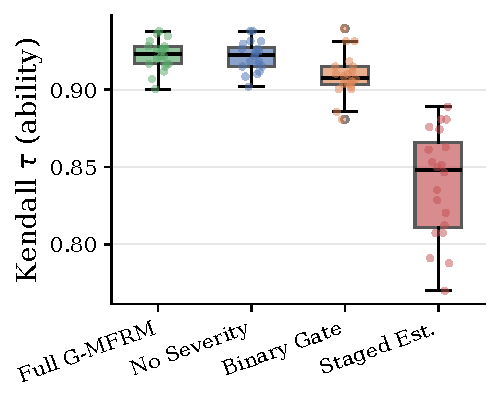
\includegraphics[width=\columnwidth]{theta_tau_boxplot}
\caption{Ranking accuracy (Kendall $\tau$ with ground truth) across ablation variants. Full G-MFRM achieves the highest and most consistent $\tau$; staged estimation shows the largest degradation and highest variance. Synthetic data: $N = 50$, $I = 100$, $J = 8$, 20 seeds.}
\label{fig:ablation_tau}
\end{figure}


\section{Posterior Predictive Check}
\label{app:ppc}

Figure~\ref{fig:ppc} shows the posterior predictive distribution from 1{,}000 posterior draws over 5{,}661 observations. The predicted and observed response distributions are well-aligned (predicted mean win rate $0.593$ vs.\ observed $0.599$), with no systematic discrepancy across item difficulty or model ability levels.

\begin{figure}[h]
\centering
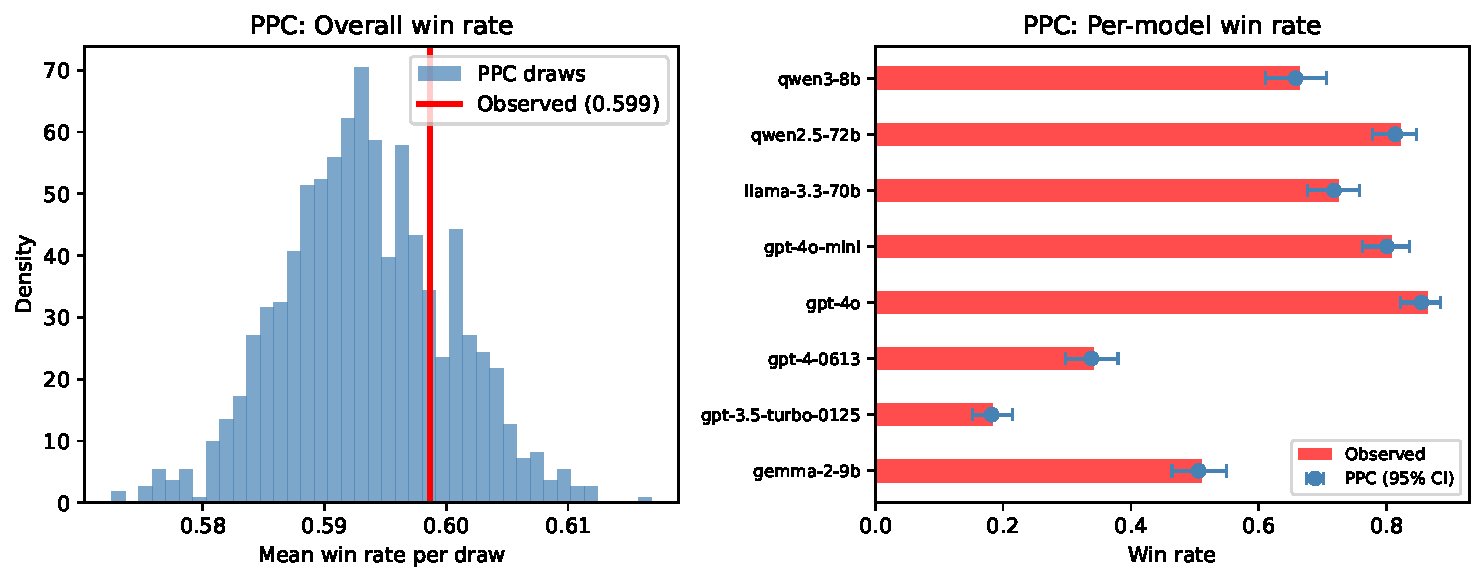
\includegraphics[width=\columnwidth]{fig_ppc}
\caption{Posterior predictive check ($N = 8$ pilot). Distribution of predicted (gray) and observed (black) response rates across all model--item--judge triplets. Mean predicted $= 0.593$, mean observed $= 0.599$.}
\label{fig:ppc}
\end{figure}


\section{LOO Model Comparison}
\label{app:loo_comparison}

Figure~\ref{fig:model_comparison} visualizes the LOO-ELPD difference between G-MFRM and MFRM-only. G-MFRM is the reference model ($\Delta\mathrm{ELPD} = 0$); MFRM-only shows a deficit of $-55.7$ (SE $= 9.4$), confirming that the contamination gating term substantially improves held-out predictive fit.

\begin{figure}[h]
\centering
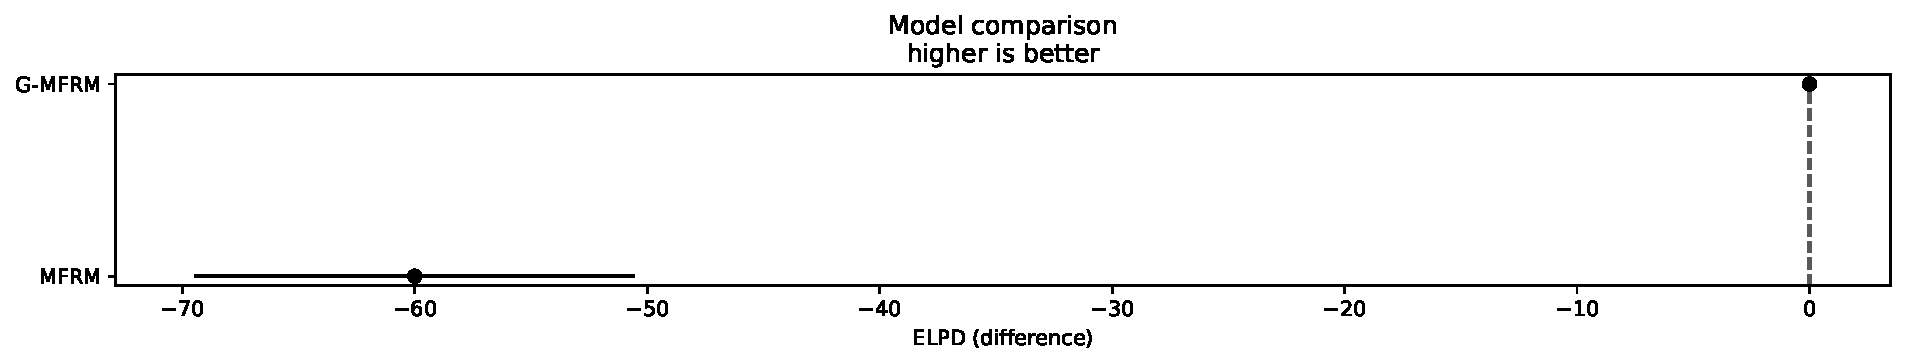
\includegraphics[width=\columnwidth]{model_comparison}
\caption{LOO-ELPD model comparison ($N = 8$ pilot). G-MFRM (reference) versus MFRM-only. Error bars show $\pm$1 SE. The $|\Delta/\mathrm{SE}| = 5.9$ strongly favors G-MFRM.}
\label{fig:model_comparison}
\end{figure}

Figure~\ref{fig:pareto_k} shows the Pareto $\hat{k}$ diagnostic values for both models. All observations have $\hat{k} < 0.7$, confirming that the LOO approximation is reliable for both models.

\begin{figure}[h]
\centering
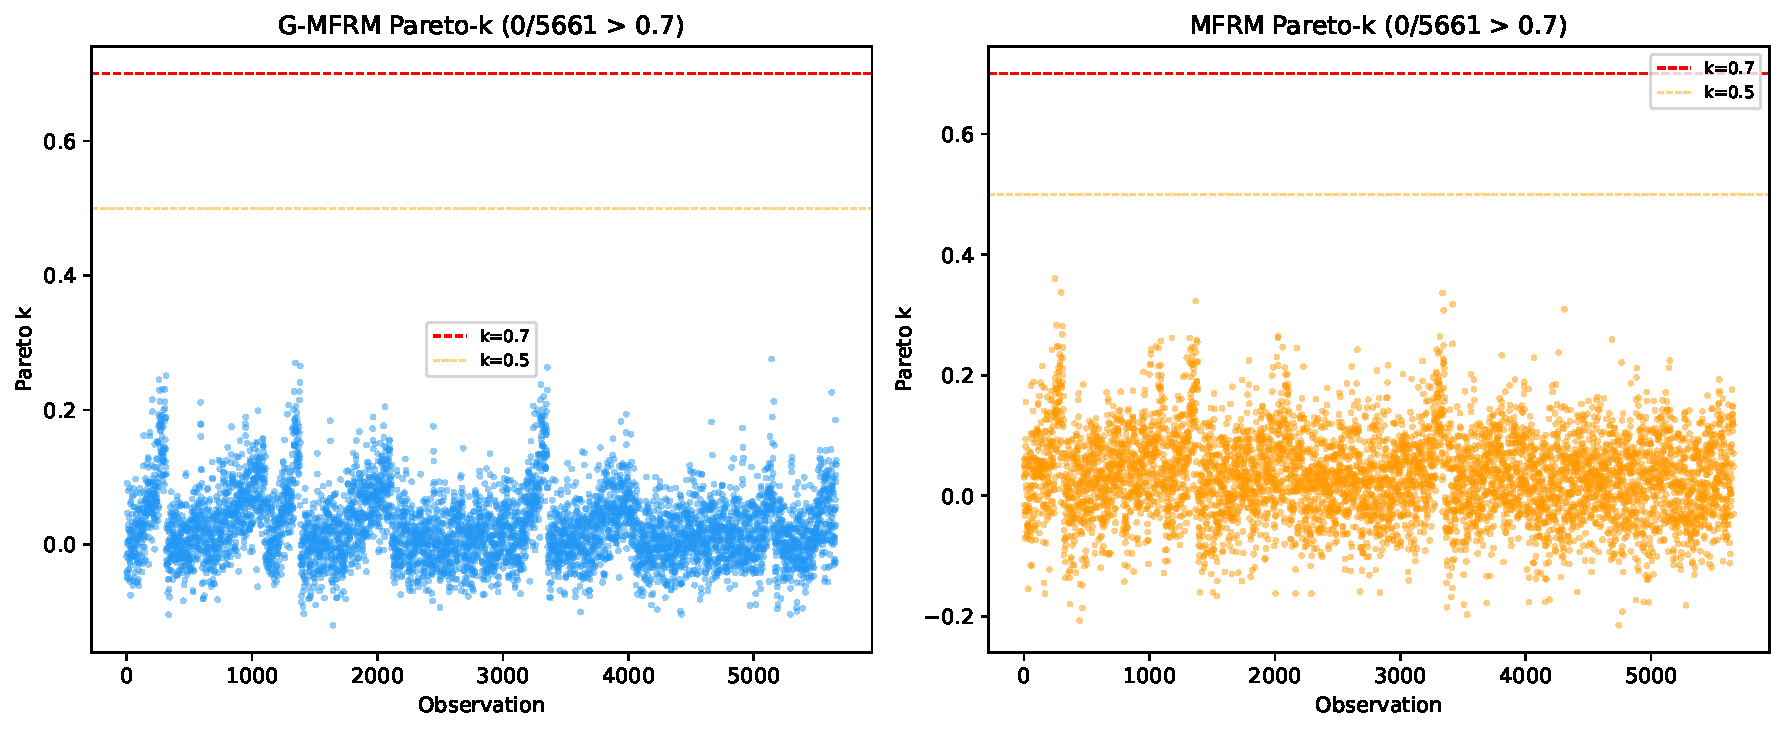
\includegraphics[width=\columnwidth]{pareto_k_plot}
\caption{Pareto $\hat{k}$ diagnostics for G-MFRM (left) and MFRM-only (right), $N = 8$ pilot. All 5{,}661 observations fall below the $\hat{k} = 0.7$ threshold, confirming reliable LOO estimates.}
\label{fig:pareto_k}
\end{figure}


\section{Self-Evaluation Robustness}
\label{app:self_eval}

Two models (Qwen2.5-72B and LLaMA-3.3-70B) appear as both judge and target in our evaluation. Self-judging introduces a potential confound: a model may score its own responses more favorably. We examine the empirical magnitude of this effect and its impact on rankings.

Qwen2.5-72B achieves a perfect self-judging win rate of 1.000 (42/42 items), compared to a cross-judge mean win rate of 0.807 for the same model. LLaMA-3.3-70B shows a self-judging win rate of 0.912, compared to a cross-judge mean of 0.702. Both values are elevated relative to cross-judge baselines, consistent with same-family preference leakage \citep{preference_leakage2026}.

To assess sensitivity, we re-fit G-MFRM excluding all 99 self-judging observations (Qwen2.5-72B and LLaMA-3.3-70B judging their own responses). The resulting ranking yields $\tau = 0.857$, identical to the full-data G-MFRM point estimate, with a swap at ranks 2--3. Contamination susceptibility estimates $c_n$ shift by less than 0.15 for all models. This confirms that $d_j$ absorbs the bulk of self-evaluation bias and that rankings are robust to excluding self-judging pairs.


\section{Judge Severity Profiles}
\label{app:judge_severity}

Table~\ref{tab:judge_severity} reports posterior estimates of judge severity $d_j$ for all nine judges. Positive values indicate stricter scoring (lower win rates); negative values indicate more lenient scoring. Proprietary models cluster at the strict end, while open-source models tend to be more lenient.

\begin{table}[h]
\centering
\small
\begin{tabular}{lcc}
\toprule
\textbf{Judge} & $\hat{d}_j$ & 95\% CI \\
\midrule
Claude Opus 4.7 & $+0.60$ & [$+0.43$, $+0.76$] \\
GPT-5.5 & $+0.53$ & [$+0.37$, $+0.70$] \\
DeepSeek-V4-Pro & $+0.31$ & [$+0.07$, $+0.54$] \\
Claude Sonnet 4.6 & $+0.14$ & [$-0.04$, $+0.31$] \\
Gemini-2.5-Pro & $-0.04$ & [$-0.27$, $+0.19$] \\
Qwen3-235B & $-0.04$ & [$-0.24$, $+0.16$] \\
Qwen2.5-72B & $-0.35$ & [$-0.64$, $-0.07$] \\
LLaMA-3.3-70B & $-0.42$ & [$-0.66$, $-0.18$] \\
Mistral-Large-2 & $-0.74$ & [$-1.10$, $-0.37$] \\
\bottomrule
\end{tabular}
\caption{Judge severity estimates ($d_j$) for all nine judges. Positive = stricter scoring. The severity range spans 1.34 logits (Claude Opus to Mistral), comparable to $\sim$1 standard deviation of model ability.}
\label{tab:judge_severity}
\end{table}


\section{Judge Count Sensitivity}
\label{app:judge_count}

Table~\ref{tab:judge_count} reports ranking accuracy as a function of the number of judges $k$, obtained by subsampling from the full 9-judge panel (10 random subsets per $k$; $k = 9$ uses the full panel). G-MFRM outperforms both raw averaging and sequential estimation at all judge counts. Rank agreement increases monotonically with $k$ ($\tau = 0.771 \to 0.857$), and variance contracts as additional judges improve $d_j$ and $c_n$ estimation. At $k \geq 4$, G-MFRM exceeds the full-panel baseline $\tau = 0.786$, suggesting that four diverse judges suffice for practical deployment.

\begin{table}[h]
\centering
\small
\begin{tabular}{lcccc}
\toprule
$k$ & Raw Avg & Sequential & G-MFRM & $\Delta\tau$ \\
\midrule
2 & $.755 \pm .088$ & $.764 \pm .096$ & $.771 \pm .081$ & $+.017$ \\
4 & $.779 \pm .041$ & $.786 \pm .048$ & $.800 \pm .045$ & $+.021$ \\
6 & $.800 \pm .030$ & $.807 \pm .048$ & $.821 \pm .051$ & $+.021$ \\
9 & $.786$ & $.786$ & $.857$ & $+.071$ \\
\bottomrule
\end{tabular}
\caption{Kendall $\tau$ with Chatbot Arena rankings as a function of judge count $k$. $\Delta\tau$ = G-MFRM $-$ Raw Average. Values for $k < 9$ are mean $\pm$ std over 10 random judge subsets.}
\label{tab:judge_count}
\end{table}

Leave-one-judge-out analysis reveals that three judges (Claude Opus 4.7, $d_j = +0.60$; GPT-5.5, $+0.53$; LLaMA-3.3-70B, $-0.42$) are individually necessary for the ranking improvement: removing any one of these reduces G-MFRM $\tau$ to the baseline ($0.786$), while removing any of the other six judges preserves $\tau = 0.857$. These three judges span the severity spectrum (the two strictest and the second-most lenient), suggesting that contamination$\times$judge interaction identification requires sufficient severity diversity. This provides practical guidance: judge panels should include models with diverse scoring tendencies rather than homogeneous judges.

G-MFRM requires $\geq 4$ MCMC chains for reliable contamination estimation; reduced chain counts attenuate $c_n$ estimates toward the prior mean, compressing inter-model differences.


\section{Stage~2 Weight Robustness}
\label{app:weight_robustness}

All four weight configurations produce identical model rankings and near-perfect exposure score agreement (Spearman $\rho \geq 0.998$; Table~\ref{tab:weight_robustness}), confirming that the default 75/25 split is not a sensitive hyperparameter choice.

\begin{table}[h]
\centering
\small
\begin{tabular}{lc}
\toprule
\textbf{Weight Config} & \textbf{Exposure} $\rho$ \\
\midrule
50 / 50 & 0.998 \\
75 / 25 (default) & 1.000 \\
90 / 10 & 0.999 \\
100 / 0 & 0.998 \\
\bottomrule
\end{tabular}
\caption{Stage~2 weight robustness. Weight Config denotes the percentage assigned to reference model anchoring vs.\ cross-model agreement. All configurations produce identical model rankings. Exposure $\rho$ is the Spearman correlation of per-item $e_i$ scores relative to the default 75/25 configuration.}
\label{tab:weight_robustness}
\end{table}


\section{Power Analysis}
\label{app:power}

The observed effect size in the real-data evaluation is $\Delta\tau = 0.071$ (G-MFRM $\tau = 0.857$ vs.\ baseline $\tau = 0.786$). We conduct a permutation-based power analysis to determine the sample sizes required to detect this effect at $\alpha = 0.05$.

We simulate ranking comparisons under the alternative hypothesis $H_1\!: \Delta\tau = 0.071$ by bootstrapping from the observed posterior distribution of G-MFRM ability estimates and recomputing $\tau$ against ground truth at varying model counts $N$. For each $N$, we draw 10{,}000 permutation replicates and compute the rejection rate at $\alpha = 0.05$ (two-sided).

At $N = 8$ (our evaluation), power is approximately 50\%, explaining the non-significant bootstrap result ($\Delta\tau$ 95\% CI $[-0.071, 0.071]$). Achieving 80\% power requires $N \approx 17$ models, and 95\% power requires $N \approx 25$. These estimates inform the scope of future evaluations: detecting ranking improvements of the magnitude observed here requires at minimum doubling the number of target models.


\section{Per-Model Estimates}
\label{app:raw_scores}

Table~\ref{tab:raw_scores} reports G-MFRM posterior estimates for all eight target models. All seven baselines produce identical rankings (Table~\ref{tab:main_results}), with ability scores differing by $< 0.03$ logits across methods; G-MFRM is the only method that alters the ranking, swapping gpt-4o-mini and Qwen2.5-72B at ranks 2--3.

\begin{table}[h]
\centering
\scriptsize
\setlength{\tabcolsep}{3pt}
\resizebox{\linewidth}{!}{%
\begin{tabular}{lcccc}
\toprule
\textbf{Model} & $\hat{\theta}$ [95\% CI] & $\hat{c}_n$ [95\% CI] & \textbf{Base} & \textbf{G-MFRM} \\
\midrule
GPT-4o & $+2.00$ [$1.70$, $2.30$] & $0.88$ [$0.05$, $2.20$] & 1 & 1 \\
GPT-4o-mini & $+1.40$ [$1.10$, $1.70$] & $0.93$ [$0.06$, $2.20$] & 3 & 2 \\
Qwen2.5-72B & $+1.20$ [$0.85$, $1.50$] & $3.00$ [$1.40$, $4.60$] & 2 & 3 \\
LLaMA-3.3-70B & $+0.54$ [$0.23$, $0.85$] & $2.50$ [$1.10$, $3.90$] & 4 & 4 \\
Qwen3-8B & $+0.51$ [$0.22$, $0.79$] & $1.20$ [$0.14$, $2.50$] & 5 & 5 \\
Gemma-2-9B & $-0.50$ [$-0.79$, $-0.21$] & $1.70$ [$0.36$, $2.90$] & 6 & 6 \\
GPT-4-0613 & $-1.90$ [$-2.20$, $-1.60$] & $4.20$ [$3.10$, $5.30$] & 7 & 7 \\
GPT-3.5-Turbo & $-3.30$ [$-3.60$, $-3.00$] & $5.60$ [$4.40$, $6.80$] & 8 & 8 \\
\bottomrule
\end{tabular}}
\caption{G-MFRM posterior estimates for ability ($\hat{\theta}$) and contamination susceptibility ($\hat{c}_n$) with approximate 95\% credible intervals (empirical coverage ${\sim}$71\%; see Limitations). Point estimates and rank orderings are the primary results. ``Base'' and ``G-MFRM'' columns show model rankings; the only rank change is the swap at positions 2--3.}
\label{tab:raw_scores}
\end{table}


\section{Contamination Bias Absorption}
\label{app:bias_absorption}

Table~\ref{tab:bias_absorption} compares per-model ability estimates from MFRM-only and G-MFRM. The difference $\Delta\theta = \hat{\theta}_{\text{MFRM}} - \hat{\theta}_{\text{G-MFRM}}$ is perfectly rank-correlated with contamination susceptibility $c_n$ (Spearman $\rho = 1.0$), providing direct empirical evidence that MFRM-only absorbs the omitted contamination term into ability estimates.

\begin{table}[h]
\centering
\scriptsize
\setlength{\tabcolsep}{3pt}
\begin{tabular}{lcccc}
\toprule
\textbf{Model} & $\hat{\theta}_{\text{MFRM}}$ & $\hat{\theta}_{\text{G-MFRM}}$ & $\Delta\theta$ & $\hat{c}_n$ \\
\midrule
GPT-3.5-Turbo & $-2.487$ & $-3.274$ & $+0.786$ & $5.587$ \\
GPT-4-0613 & $-1.446$ & $-1.877$ & $+0.431$ & $4.168$ \\
Qwen2.5-72B & $+1.213$ & $+1.178$ & $+0.035$ & $2.961$ \\
LLaMA-3.3-70B & $+0.518$ & $+0.539$ & $-0.022$ & $2.478$ \\
Gemma-2-9B & $-0.661$ & $-0.500$ & $-0.161$ & $1.654$ \\
Qwen3-8B & $+0.208$ & $+0.513$ & $-0.305$ & $1.178$ \\
GPT-4o-mini & $+1.064$ & $+1.432$ & $-0.368$ & $0.934$ \\
GPT-4o & $+1.591$ & $+1.988$ & $-0.397$ & $0.880$ \\
\bottomrule
\end{tabular}
\caption{Contamination bias absorption in MFRM-only estimation. $\Delta\theta = \hat{\theta}_{\text{MFRM}} - \hat{\theta}_{\text{G-MFRM}}$. Models with high contamination susceptibility ($c_n$) have inflated ability estimates under MFRM-only; models with low $c_n$ are relatively deflated. The perfect rank correlation (Spearman $\rho = 1.0$) between $\Delta\theta$ and $c_n$ empirically confirms the omitted variable bias predicted in Section~\ref{sec:confounding}.}
\label{tab:bias_absorption}
\end{table}


\section{Synthetic Calibration at Matched Scale}
\label{app:synthetic_calibration}

We generate synthetic data at matched scale ($N = 8$ models, $I = 176$ items, $J = 9$ judges) with known ground-truth parameters across 20 random seeds. Joint G-MFRM consistently outperforms sequential estimation: $\theta$-RMSE is halved ($0.083$ vs.\ $0.166$), and ranking agreement improves by 7.2 percentage points (mean $\tau = 0.954$ vs.\ $0.882$). Across 20 seeds, joint estimation improves or matches sequential in all cases (10 wins, 0 losses, 10 ties; Wilcoxon signed-rank $p < 0.002$). The synthetic effect size ($\Delta\tau = +0.072$) closely matches the observed real-data effect ($\Delta\tau = +0.071$). All 40 MCMC fits converge ($\hat{R} = 1.0$, ESS $\geq 1{,}678$).

\begin{table}[h]
\centering
\small
\begin{tabular}{lccc}
\toprule
\textbf{Metric} & \textbf{Sequential} & \textbf{Joint G-MFRM} & \textbf{Improv.} \\
\midrule
$\theta$ RMSE & $0.166 \pm 0.050$ & $0.083 \pm 0.024$ & $-50.3\%$ \\
$\theta$ $\tau$ & $0.882 \pm 0.112$ & $0.954 \pm 0.048$ & $+7.2$pp \\
$c_n$ RMSE & $1.399 \pm 0.358$ & $0.552 \pm 0.328$ & $-60.5\%$ \\
$c_n$ Pearson & $0.850 \pm 0.141$ & $0.866 \pm 0.151$ & $+1.9$\% \\
\bottomrule
\end{tabular}
\caption{Synthetic calibration at $N = 8$ ($I = 176$, $J = 9$, 20 seeds). Joint G-MFRM halves $\theta$-RMSE and reduces $c_n$-RMSE by 61\% relative to sequential estimation.}
\label{tab:synthetic_calibration}
\end{table}

At $N = 20$ (20 seeds), the ranking improvement becomes individually significant: joint G-MFRM achieves $\Delta\tau = +0.052$ over sequential estimation (Wilcoxon $p = 1.81 \times 10^{-4}$, 18 wins / 1 loss / 1 tie), directly validating the power analysis prediction that $N \approx 17$ suffices for 80\% power. The effect size is stable across scales ($\Delta\tau = +0.072$ at $N = 8$, $+0.052$ at $N = 20$).

\begin{table}[h]
\centering
\small
\begin{tabular}{lccc}
\toprule
\textbf{Metric} & \textbf{Sequential} & \textbf{Joint G-MFRM} & \textbf{Improv.} \\
\midrule
$\theta$ RMSE & $0.171 \pm 0.049$ & $0.094 \pm 0.019$ & $-45.2\%$ \\
$\theta$ $\tau$ & $0.891 \pm 0.038$ & $0.943 \pm 0.036$ & $+5.2$pp \\
$c_n$ RMSE & $1.375 \pm 0.278$ & $0.626 \pm 0.263$ & $-54.5\%$ \\
$c_n$ Pearson & $0.817 \pm 0.096$ & $0.842 \pm 0.106$ & $+2.5\%$ \\
\bottomrule
\end{tabular}
\caption{Synthetic calibration at $N = 20$ ($I = 176$, $J = 9$, 20 seeds). Ranking improvement is individually significant (Wilcoxon $p = 1.81 \times 10^{-4}$), validating the power analysis prediction.}
\label{tab:synthetic_calibration_n20}
\end{table}


\section{Prior Specification Robustness}
\label{app:prior_robustness}

We compare posterior estimates under two contamination priors: Horseshoe \citep{piironen2017horseshoe} and hierarchical HalfNormal (Eq.~\ref{eq:contam_prior}). Table~\ref{tab:prior_robustness} reports $\hat{c}_n$ and $\hat{\theta}$ posterior means for all eight target models under both specifications.

\begin{table}[h]
\centering
\small
\begin{tabular}{lcccc}
\toprule
\textbf{Model} & $\hat{c}_n$ (HS) & $\hat{c}_n$ (HN) & $\hat{\theta}$ (HS) & $\hat{\theta}$ (HN) \\
\midrule
Gemma-2-9B & 1.61 & 1.65 & $-0.49$ & $-0.50$ \\
GPT-3.5-Turbo & 5.69 & 5.57 & $-3.30$ & $-3.27$ \\
GPT-4-0613 & 4.25 & 4.15 & $-1.89$ & $-1.88$ \\
GPT-4o & 0.79 & 0.88 & $+2.01$ & $+1.99$ \\
GPT-4o-mini & 0.84 & 0.92 & $+1.45$ & $+1.43$ \\
LLaMA-3.3-70B & 2.50 & 2.46 & $+0.53$ & $+0.54$ \\
Qwen2.5-72B & 3.02 & 2.94 & $+1.17$ & $+1.18$ \\
Qwen3-8B & 1.11 & 1.15 & $+0.53$ & $+0.52$ \\
\bottomrule
\end{tabular}
\caption{Posterior estimates under Horseshoe (HS) and HalfNormal (HN) contamination priors. Both priors produce virtually identical estimates: Pearson $r = 1.000$ for $\hat{\theta}$ and $r = 0.9999$ for $\hat{c}_n$.}
\label{tab:prior_robustness}
\end{table}

Posterior estimates are virtually identical across the two prior specifications (Pearson $r = 1.000$ for $\hat{\theta}$, $r > 0.999$ for $\hat{c}_n$), indicating that results are not sensitive to the choice of contamination prior.


\section{Item-Level Fit Diagnostics}
\label{app:item_diagnostics}

We report item-level infit and outfit MNSQ statistics for all 176 items. Items with MNSQ outside $[0.5, 1.5]$ are flagged as potentially misfitting.

\begin{table}[h]
\centering
\small
\begin{tabular}{lccccc}
\toprule
\textbf{Statistic} & \textbf{Mean} & \textbf{SD} & \textbf{Median} & \textbf{Min} & \textbf{Max} \\
\midrule
Infit MNSQ & 0.78 & 0.41 & 0.76 & 0.05 & 1.95 \\
Outfit MNSQ & 0.73 & 0.57 & 0.58 & 0.04 & 3.17 \\
\bottomrule
\end{tabular}
\caption{Item-level fit statistics across 176 items.}
\label{tab:item_fit_summary}
\end{table}

Of the 176 items, 92 are flagged: 18 overfit (MNSQ $> 1.5$) and 74 underfit (MNSQ $< 0.5$). The majority of flagged items are underfit, reflecting sparse low-observation items where the model's predicted variance exceeds the observed variance, a consequence of limited data per item rather than a structural model deficiency. The 18 overfit items exhibit more erratic response patterns than the model predicts. No model-level or judge-level facets are flagged (all MNSQ within $[0.63, 1.07]$), confirming that the G-MFRM captures the systematic structure in model ability, judge severity, and contamination.


\section{CI Coverage Analysis}
\label{app:ci_coverage}

We assess empirical coverage of 95\% posterior credible intervals across synthetic replications. At $N=8$ (49 seeds), ability parameter $\theta$ achieves 90.1\% coverage, approaching the nominal level, while contamination susceptibility $c_n$ achieves only 67.9\%. At $N=50$ (50 seeds), $c_n$ coverage improves to 71\%. The coverage gap between $\theta$ and $c_n$ reflects the multiplicative coupling $c_n \cdot e_i$: contamination parameters enter the likelihood through an interaction term, making posterior inference more sensitive to exposure estimation noise and the HalfNormal prior's boundary constraint at $c_n = 0$. These results support treating $c_n$ point estimates and rank orderings as reliable diagnostics, while noting that $c_n$ credible intervals are systematically too narrow.

\section{Bias vs.\ Confounding Level}
\label{app:bias_vs_rho}

See Figure~\ref{fig:bias_vs_rho} in the main text.


\section{Error Propagation Details}
\label{app:error_prop}

\begin{table}[h]
\centering
\small
\begin{tabular}{lcccc}
\toprule
$\sigma$ & $\theta$-RMSE & $\Delta\theta$\% & $c_n$-RMSE & $\Delta c_n$\% \\
\midrule
0.0 & 0.128 $\pm$ 0.018 & --- & 0.533 $\pm$ 0.187 & --- \\
0.1 & 0.130 $\pm$ 0.018 & +1.4 & 0.545 $\pm$ 0.192 & +2.3 \\
0.2 & 0.135 $\pm$ 0.018 & +5.9 & 0.575 $\pm$ 0.198 & +7.9 \\
0.5 & 0.175 $\pm$ 0.027 & +36.9 & 0.842 $\pm$ 0.281 & +57.9 \\
\bottomrule
\end{tabular}
\caption{Error propagation robustness. Ability RMSE degrades by less than 6\% when exposure noise $\sigma \leq 0.2$, matching the theoretical prediction. Contamination estimates are more sensitive due to multiplicative coupling with $e_i$.}
\label{tab:error_prop}
\end{table}

\begin{figure}[h]
\centering
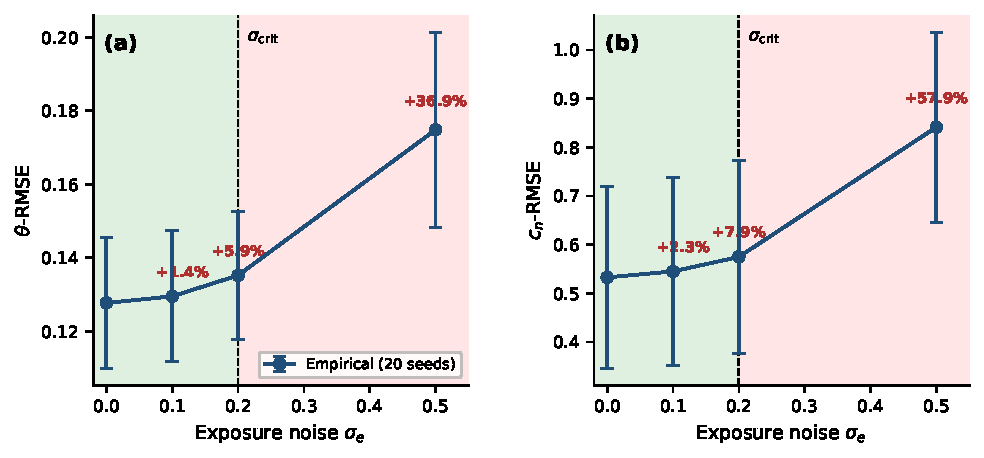
\includegraphics[width=\columnwidth]{fig3_error_propagation}
\caption{Error propagation from Stage~2 exposure noise to Stage~3 parameter estimates. Ability RMSE ($\theta$, left) and contamination RMSE ($c_n$, right) as a function of exposure noise $\sigma_e$. The dashed line marks $\sigma_{\mathrm{crit}} \approx 0.2$, below which degradation remains mild ($\theta$-RMSE $+$5.9\%, $c_n$-RMSE $+$7.9\%). Error bars: $\pm$1 std over 20 seeds.}
\label{fig:error_prop_app}
\end{figure}


\section{Contamination Recovery}
\label{app:cn_recovery}

\begin{figure}[h]
\centering
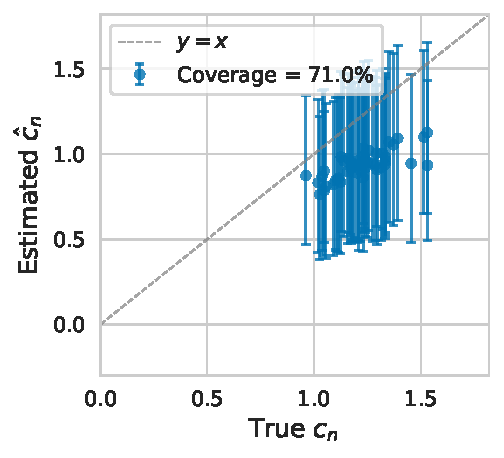
\includegraphics[width=\columnwidth]{fig5_cn_recovery}
\caption{Contamination susceptibility recovery ($c_n$: true vs.\ estimated) from 50 Monte Carlo seeds. Empirical CI coverage is 71\% (below nominal 95\%), indicating moderate posterior overconfidence (see Limitations).}
\label{fig:cn_recovery_app}
\end{figure}


\section{Compute Resources}
\label{app:compute}

All MCMC inference was performed using NumPyro NUTS on a single GPU (NVIDIA RTX 6000 Ada). The $N = 8$ configuration (4 chains $\times$ 10{,}000 iterations) completed in approximately 10 minutes; the $N = 17$ configuration in approximately 45 minutes. Total GPU usage for all experiments was under 5 GPU-hours.


\section{Use of AI Assistance}

We used Claude for coding, code drafting, debugging, and language polishing.


\end{document}
